\section{Academic Figures and Deterministic Geometric Evaluation}\label{sec:geometric}

AI-generated SVG and architecture figures for papers routinely exhibit
\emph{geometric} defects: text labels that overlap one another, boxes clipped at
the canvas edge, text overflowing its container, or content that pushes the
document past its intended bounds. These are precisely the kind of layout flaws a
render-and-review loop ought to detect and repair. To study this, we introduce a
seventh modality, beyond the six harness modalities of \Cref{sec:harness}: a
geometry-focused Type-3b suite of 20 dense academic-paper architecture figures
(Transformer, U-Net, ViT, Swin, FPN, DETR, Mask R-CNN, Faster R-CNN,
latent-diffusion U-Net, CLIP, MoE, GAT, WaveNet, SE, Perceiver-IO, Seq2Seq with
attention, Flamingo, Evoformer, $\dots$), each generated as a self-contained
$1920\times1080$ HTML document with inline SVG, and each hardened with a legend
and per-block tensor-shape annotations so a frontier model cannot trivially lay
it out. The defining property of these artifacts is that correctness is largely
\emph{geometric}: whether the components are present and wired correctly is
semantic, but whether the figure is actually legible is a question of spatial
layout that can be measured exactly. This modality therefore
serves as a clean testbed for whether our evaluation instrument can perceive the
defects that an interaction loop is supposed to fix.

\subsection{VLM screenshot judging is unreliable for geometric defects}

Our default visual evaluator is a binary per-requirement rubric scored by a
vision--language model (VLM) over a screenshot of the rendered artifact. Even
when we capture the screenshot at native resolution and tile it into quadrants to
preserve detail, on an initial 15-figure probe this judge scored \textbf{14 of
15} single-shot figures as perfect. Yet by direct inspection the figures are plainly broken: the Evoformer
figure renders two section titles, ``MSA Processing'' and ``MSA
Representation,'' superimposed on top of one another, and the ViT figure's detail
panel has ``Class Output'' overlapping ``Input.'' The judge cannot see these
defects, and the reason is mechanical: screenshots are captured at $1080$ pixels
of height, so any content that overflows the canvas is cropped \emph{off-frame}
before the image ever reaches the VLM. The most severe geometric failures---those
that push content past the viewport---are exactly the ones the screenshot cannot
contain, and small overlaps that do remain in-frame fall below the VLM's
effective acuity. A VLM scoring a single fixed-resolution capture is
structurally blind to overflow and to fine-grained overlap, which is why the
correct instrument for fixed-canvas visual artifacts measures the rendered
layout directly rather than a picture of it.

\subsection{Deterministic geometry}

To obtain a reliable instrument we replace the VLM with a deterministic
DOM-geometry checker. The checker loads the HTML document in a headless browser
and, via the page's own layout engine, extracts the bounding box of every
rendered element. From these boxes it computes, exactly and reproducibly:
\emph{(i)} text-box overlaps---pairs of non-nested text elements whose boxes
intersect (at a $6$\,px threshold); \emph{(ii)} out-of-bounds content---text or
SVG primitives clipped at the viewport edge; \emph{(iii)} overflow---text
extending past its containing box; and \emph{(iv)} document overflow---the
document exceeding $1920\times1080$ by more than $16$\,px, the margin chosen to
filter spurious default browser margins. Each of these is an objective predicate
on the rendered DOM, with no model in the loop and no dependence on screenshot
framing; a VLM is needed only for the genuinely semantic axes (are the right
components present and correctly wired). Under this checker, only \textbf{3 of
15} single-shot figures are geometrically clean, with a mean of $1.6$ defects per
figure---in direct contradiction to the VLM's $14/15$ ``perfect.'' The
deterministic metric perceives the very defects to which the VLM is blind.

\subsection{Interaction scaling on an objective metric}

With a reliable instrument in hand we can measure whether the interaction loop
actually improves the artifact. The harness is fully deterministic: a proposer
generates the artifact, the DOM checker computes its exact set of geometric
defects, those specific defects are fed back to the proposer in natural language
(e.g., ``text $X$ overlaps text $Y$; move them apart''; ``the panels in this row
are unequal width; equalize and align them''; ``content is $80$\,px too wide at
$375$\,px''), and the proposer revises, for up to three iterations. The reward is
simply the defect count---no VLM is involved at any point.

We extend the checker with a deterministic \emph{alignment} axis (groups of
card/pillar boxes flagged for unequal size, misaligned far edges, or uneven
gutters), since rows of equal-width, edge-aligned panels are the failure mode that
dominates dense slides and web layouts, and we evaluate three visual modalities
under one identical configuration: Claude Sonnet 4 at temperature $0$, the same
design-principle generation prompt, the alignment-inclusive geometric reward, and
three seeds each. The three suites are $20$ dense academic-paper architecture
figures, $12$ slides that reproduce the content of well-known papers
(Transformer, ResNet, BERT, U-Net, $\dots$) with dense text coexisting with a
figure and aligned pillars, and $20$ dense responsive web pages (dashboards,
pricing comparisons, calendars, spec sheets, $\dots$; \Cref{sec:web-geometry}).

\Cref{tab:geometric} reports the result: on all three modalities the
geometric-feedback loop produces a large, statistically significant reduction in
real layout defects, with improvements outnumbering regressions by $9$:$1$ or
better. Mean defects fall $74\%$ on figures ($0.57\to0.15$, $p=7\times10^{-4}$),
$73\%$ on dense slides ($1.25\to0.33$, $p=0.0018$), and $47\%$ on web pages
($16.1\to8.5$, $p=4\times10^{-8}$). The magnitudes track single-shot headroom:
dense responsive web pages are strikingly defect-rich out of the box ($16$ defects
per page across desktop and mobile), whereas a frontier model under a
design-principle prompt already lays out many figures and slides cleanly---so the
loop has fewer, but still significant, defects to remove.

\paragraph{The VLM is blind here, as a judge \emph{and} as a reviewer.} On the
same dense slides the binary VLM rubric saturates---it rates $29$ of $36$
single-shot slides perfect ($0.97$ mean)---while deterministic geometry finds only
half of them clean. Worse, when the \emph{reviewer} is a VLM rather than the
geometry checker, the mean slide defect count \emph{rises} ($1.89\to2.44$): blind
to the true geometry, its edits break alignment as often as they fix it. Only the
grounded geometric signal reliably removes the defects. As an independent
cross-check, re-scoring the $60$ task-runs of the \emph{original} VLM-feedback
slides harness with the DOM checker shows mean defects of $2.63\to0.23$---that
harness had been fixing real layout defects all along, but the holistic and rubric
VLM scores it reported could not measure the improvement.

\begin{figure*}[t]
  \centering
  \includegraphics[width=0.92\linewidth]{figures/comparison_grid.png}
  \caption{Single-shot (left, red) vs.\ reviewed (right, green) academic figures
  under deterministic geometric feedback. Single-shot renders are cramped and
  overflow their canvas; the interaction loop, fed the exact measured defects,
  resolves them to clean layouts. Defect counts are computed from the rendered
  DOM. Every single-shot render shown was rated ``perfect'' by the VLM screenshot
  judge.}
  \label{fig:comparison-grid}
\end{figure*}

\begin{table}[t]
  \centering
  \caption{Interaction scaling under deterministic DOM-geometry scoring, across
  three visual modalities at one identical generation configuration (Claude
  Sonnet 4, temperature $0$, design-principle prompt, alignment-inclusive
  geometric reward, three seeds; propose\,$\to$\,measure\,$\to$\,feed exact
  defects back\,$\to$\,revise, $\le 3$ iterations). Defects are counted exactly
  from the rendered DOM (text overlap, container/horizontal overflow, clipping,
  box-group misalignment); web pages are scored at desktop $1920$ and mobile
  $375$ widths and summed. Lower is better; $p$ is a two-sided paired sign test.}
  \label{tab:geometric}
  \small
  \begin{tabular}{lcccccc}
    \toprule
    Modality & $n$ & SS & Rev. & $\Delta$ & clean SS$\to$Rev. & impr./regr.\ ($p$) \\
    \midrule
    Academic figures (20) & 60 & $0.57$ & $0.15$ & $-74\%$ & $39\to52$ & $17/2$ \;($7{\times}10^{-4}$) \\
    Dense slides (12)     & 36 & $1.25$ & $0.33$ & $-73\%$ & $18\to29$ & $13/1$ \;($0.0018$) \\
    Web pages (20)        & 60 & $16.1$ & $8.5$  & $-47\%$ & $10\to16$ & $33/2$ \;($4{\times}10^{-8}$) \\
    \bottomrule
  \end{tabular}
\end{table}

\paragraph{Extending the instrument to scrollable web pages.}
\label{sec:web-geometry}
A web page has no fixed 1080-px canvas, so vertical overflow and below-the-fold
clipping are not defects---the page is meant to scroll. But the other geometric
failures are still well-defined, and a \emph{multi-width} adaptation captures the
dominant single-shot web failure: at each target width we count text-on-text
overlap, container overflow, box-group misalignment, and \emph{horizontal}
overflow (content wider than the viewport, i.e.\ a horizontal scrollbar), and we
sum these across a desktop ($1920$) and a mobile ($375$) width. The mobile pass is
what catches responsive breakage---grids that do not collapse and rows that
overflow sideways on a phone. The web row of \Cref{tab:geometric} is computed this
way, and it is the largest single-shot defect load of the three modalities ($16$
per page); notably the binary VLM rubric on the very same suite registered only a
$+0.054$ lift ($p=0.30$, n.s.), so once again the deterministic instrument reveals
a large, highly significant layout improvement that screenshot-based judging
misses entirely.

\paragraph{Scope.} Deterministic geometric scoring thus applies to any artifact
with a well-defined intended geometry: fixed-canvas slides and figures (overflow,
clipping, overlap, alignment against the canvas) and scrollable web pages (the
same predicates minus vertical overflow, evaluated per width). The binary
per-requirement rubric remains the instrument for the temporal (animation) and
factual (research) modalities, matching each artifact class to the metric that
measures it exactly.

\subsection{Binary-rubric evaluation for flowing and factual modalities}
\label{sec:rubric}

For the temporal (animation) and factual (research) modalities, and as a
complementary \emph{content} check on web pages, we score each task against its
list of concrete, independently-checkable requirements: a judge returns a binary
\textsc{satisfied}/\textsc{violated} verdict per requirement and the score is the
fraction satisfied. This multi-axis binary rubric replaces a single holistic
rating with a decomposed, reproducible measurement, and it cleanly separates a
task's individual failure modes. \Cref{tab:rubric} reports single-shot vs.\
reviewed rubric scores. On the original web suite the content rubric lifts from
$0.469$ to $0.532$ ($p=0.003$, $19$ task-runs improve and $4$ regress)---a real
but modest content gain, distinct from the large \emph{layout} gain that
deterministic multi-width geometry exposes above; on animations, from $0.642$ to
$0.834$ ($p=0.008$, $15$ improve, $3$ regress)---the largest visual-modality lift
under the rubric, as the temporal channel exposes motion defects a static rating
cannot.

\begin{table}[t]
  \centering
  \caption{Interaction scaling under binary per-requirement rubric scoring on
  the flowing visual modalities. Score is the fraction of independently-checked
  requirements satisfied; $p$ is a one-sided paired sign test over per-task-run
  deltas.}
  \label{tab:rubric}
  \begin{tabular}{lcccc}
    \toprule
    Modality (\# runs) & Feedback & Single-shot & Reviewed & sign-test $p$ \\
    \midrule
    Web pages (45)   & Type 3b (rubric)        & $0.469$ & $0.532$ & $0.003$ \\
    Animations (32)  & Type 3c (rubric)        & $0.642$ & $0.834$ & $0.008$ \\
    \bottomrule
  \end{tabular}
\end{table}

The Type-3d factual channel behaves exactly as the framework prescribes: its
lift is bounded by the model's single-shot factual error rate. On a suite of
$15$ research reports graded against web-verified ground-truth facts, a careful
single-shot report is already correct on $0.982$ of the rubric's facts, and the
search-verification loop carries it to a perfect $1.000$ with zero regressions
across all $15$ tasks. Grounded verification is precise where ungrounded review
is not: it preserves the already-correct facts rather than perturbing them, and
it corrects the residual errors it finds.

\begin{figure}[t]
  \centering
  \begin{subfigure}[t]{0.48\linewidth}
    \centering
    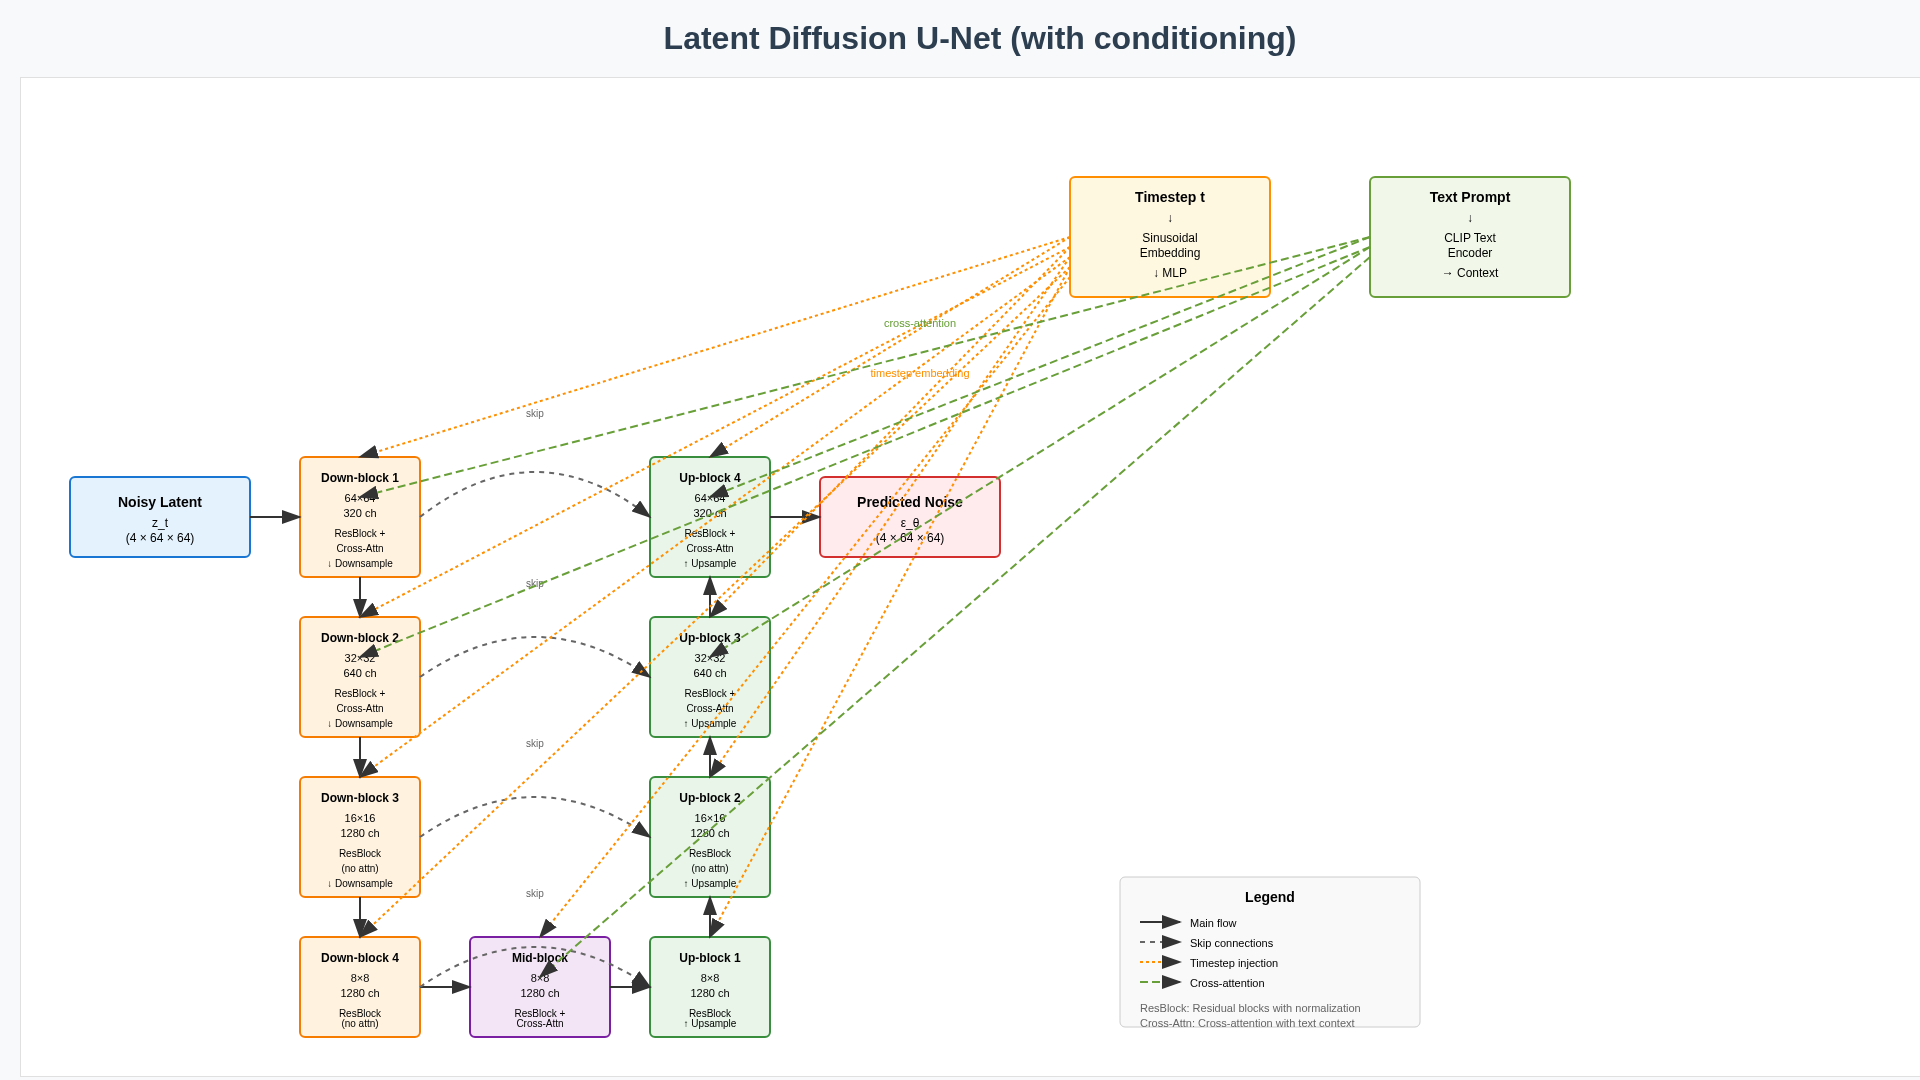
\includegraphics[width=\linewidth]{figures/diffusion_unet_singleshot.png}
    \caption{Single-shot ($4$ geometric defects).}
    \label{fig:geometric-singleshot}
  \end{subfigure}
  \hfill
  \begin{subfigure}[t]{0.48\linewidth}
    \centering
    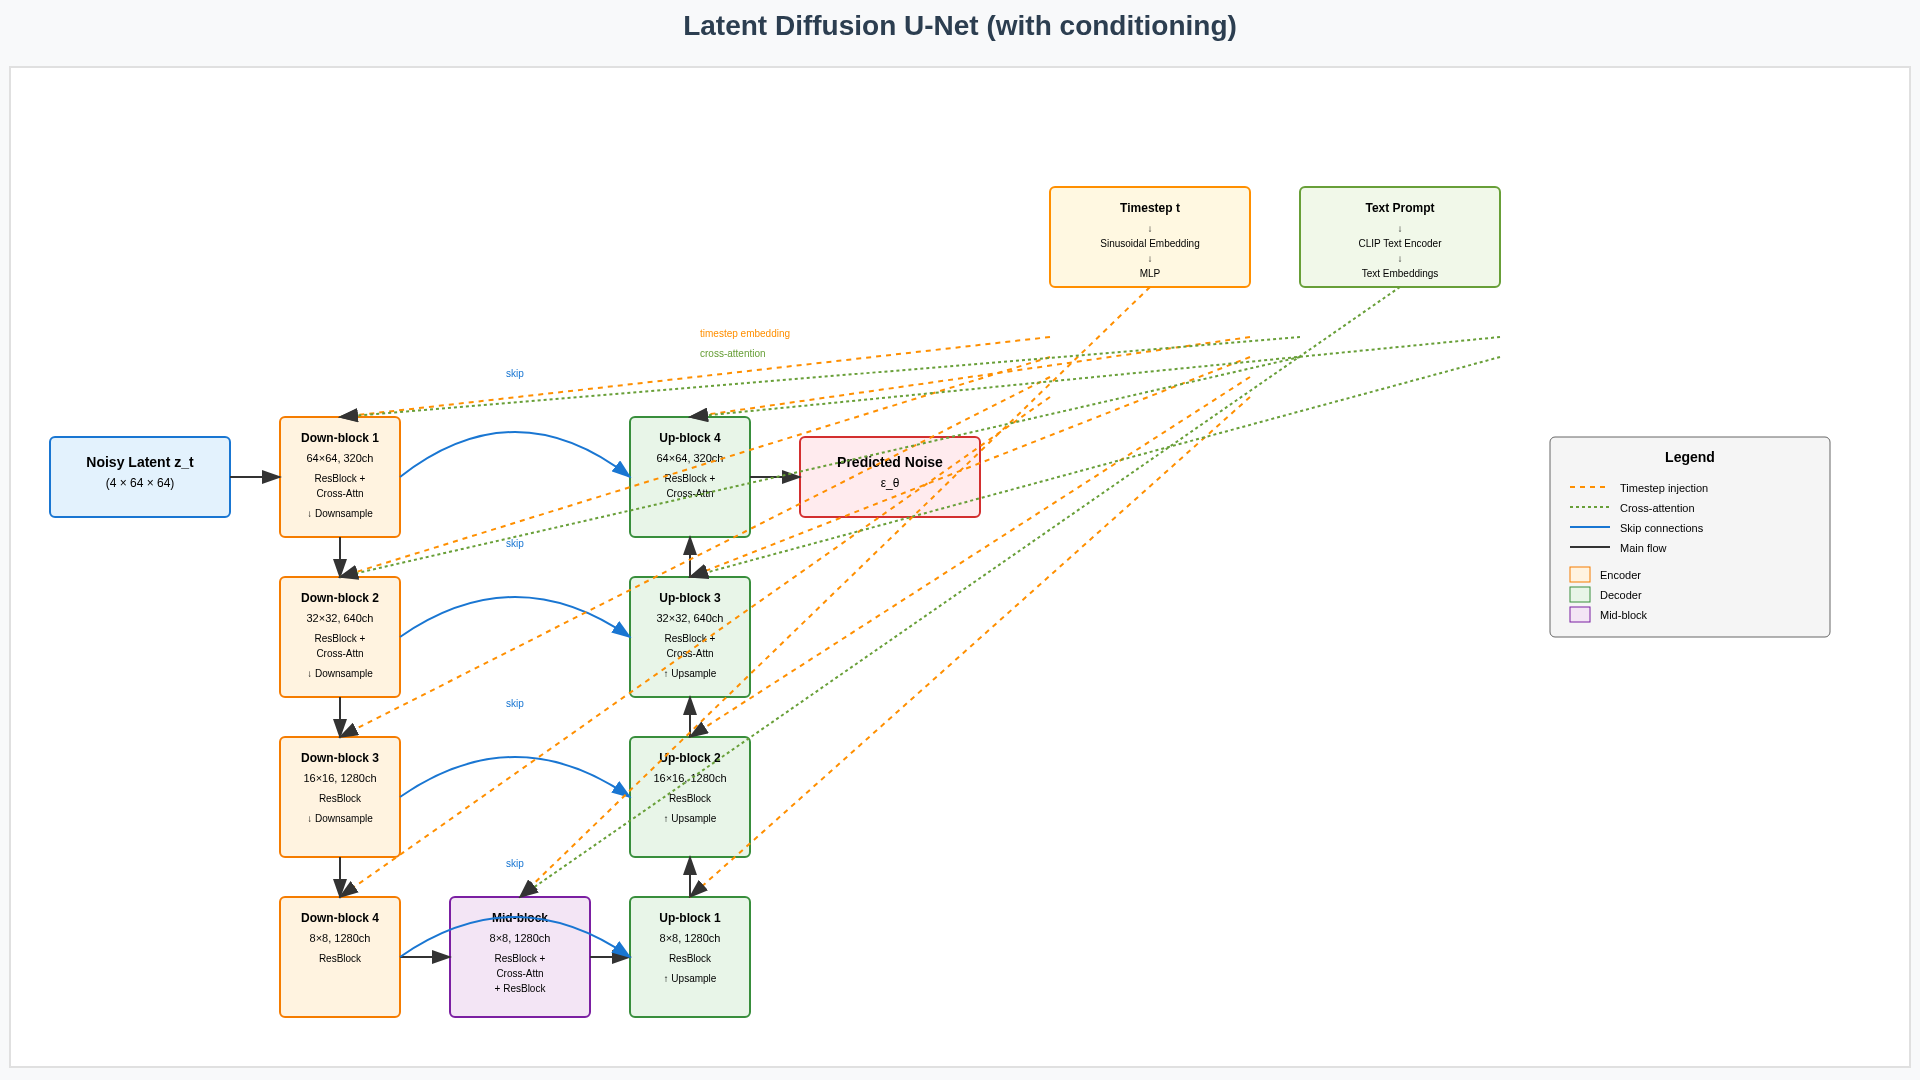
\includegraphics[width=\linewidth]{figures/diffusion_unet_reviewed.png}
    \caption{Reviewed ($0$ defects).}
    \label{fig:geometric-reviewed}
  \end{subfigure}
  \caption{The Latent Diffusion U-Net figure under deterministic geometric
  feedback. The single-shot rendering (\subref{fig:geometric-singleshot}) is
  cramped and overflows its canvas, with $4$ geometric defects that the VLM
  screenshot judge rated as perfect. After the interaction loop feeds back the
  exact defects (\subref{fig:geometric-reviewed}), the layout is clean with $0$
  defects.}
  \label{fig:geometric-beforeafter}
\end{figure}
